\section{Combinar}
\subsection{Introducción al problema}
Este filtro consiste en cambiar la distribución de píxeles de una imagen tal que queden ordenados en cuatro cuadrantes diferentes. Se obtendrá mediante la aplicación de este filtro cuatro imágenes distintas de menor tamaño a la original, pero en donde los píxeles de la original se encuentran aun presentes en la imagen resultante. Es decir : 
\begin{center}
$\forall$ $pixel,$ $cantidadPixeles(pixel, imagenOriginal) == cantidadPixeles(pixel,imagenResultante)$ 
$\wedge$ $imagenOriginal.length == imagenResultante.length$ 
\end{center}
\begin{flushright}
 $pixel \in imagenOriginal$
\end{flushright}

El resultado visual que provoca la aplicación de este filtro es la sensación de que la imagen se dividió en cuatro pequeñas imágenes cuando verdaderamente ninguna de ella es igual a la otra. 
Se puede ver en el ejemplo de la figura 1 como es la distribución que va teniendo la aplicación de nuestro filtro allí podemos distinguir que los píxeles antes y luego de la aplicación del filtro son los mismos.
\begin{figure}[H]
\begin{subfigure}[b]{0.27\textwidth}   
\centering         
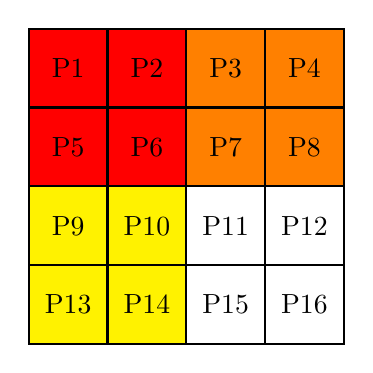
\begin{tikzpicture}
    [%%%%%%%%%%%%%%%%%%%%%%%%%%%%%%
        box/.style={rectangle,draw=black,thick, minimum size=1cm},
    ]%%%%%%%%%%%%%%%%%%%%%%%%%%%%%%
\draw[step=1cm,color=gray] (-2,-2) grid (2,2);
\node[box, fill=red] at (-1.5,+1.50) {P1};
\node[box, fill=red] at (-0.50,+1.50) {P2};
\node[box, fill=orange] at (+0.50,+1.50) {P3};
\node[box, fill=orange] at (+1.5,+1.50) {P4};
\node[box, fill=red] at (-1.5,+0.50) {P5};
\node[box, fill=red] at (-0.50,+0.50) {P6};
\node[box, fill=orange] at (+0.50,+0.50) {P7};
\node[box, fill=orange] at (+1.50,+0.50) {P8};
\node[box, fill=yellow] at (-1.50,-0.50) {P9};
\node[box, fill=yellow] at (-0.50,-0.50) {P10};
\node[box] at (+0.50,-0.50) {P11};
\node[box] at (+1.50,-0.50) {P12};
\node[box, fill=yellow] at (-1.50,-1.50) {P13};
\node[box, fill=yellow] at (-0.50,-1.50) {P14};
\node[box] at (+0.50,-1.50) {P15};
\node[box] at (+1.50,-1.50) {P16};
\end{tikzpicture}
\end{subfigure}
{\LARGE$\xrightarrow{TRANSFORMACION}$}
\begin{subfigure}[b]{0.27\textwidth} 
\centering           
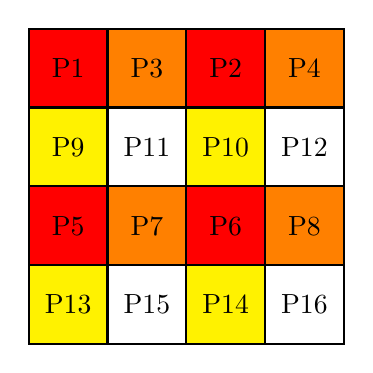
\begin{tikzpicture}
    [%%%%%%%%%%%%%%%%%%%%%%%%%%%%%%
        box/.style={rectangle,draw=black,thick, minimum size=1cm},
    ]%%%%%%%%%%%%%%%%%%%%%%%%%%%%%%
\draw[step=1cm,color=gray] (-2,-2) grid (2,2);
\node[box, fill=red] at (-1.5,+1.50) {P1};
\node[box, fill=orange] at (-0.50,+1.50) {P3};
\node[box, fill=red] at (+0.50,+1.50) {P2};
\node[box, fill=orange] at (+1.5,+1.50) {P4};
\node[box, fill=yellow] at (-1.5,+0.50) {P9};
\node[box] at (-0.50,+0.50) {P11};
\node[box, fill=yellow] at (+0.50,+0.50) {P10};
\node[box] at (+1.50,+0.50) {P12};

\node[box, fill=red] at (-1.50,-0.50) {P5};
\node[box, fill=orange] at (-0.50,-0.50) {P7};
\node[box, fill=red] at (+0.50,-0.50) {P6};
\node[box, fill=orange] at (+1.50,-0.50) {P8};

\node[box, fill=yellow] at (-1.50,-1.50) {P13};
\node[box] at (-0.50,-1.50) {P15};
\node[box, fill=yellow] at (+0.50,-1.50) {P14};
\node[box] at (+1.50,-1.50) {P16};
\end{tikzpicture}
\end{subfigure}
\caption{Distribución de píxeles tras aplicar el filtro de combinar}
\end{figure}

También podemos ver en la figura 2 cual es el impacto de nuestro filtro en una imagen real, podremos notar aqui lo parecidas que son imágenes resultantes en cada uno de los cuadrantes, a nuestro ojo es casi imperceptible la diferencia.

\begin{figure}[H]
\begin{subfigure}[b]{0.50\textwidth} 
\includegraphics[scale=0.4]{img/fourCombine_before.jpg}
\end{subfigure}
{\LARGE$\xrightarrow{T}$}
\begin{subfigure}[b]{0.50\textwidth} 
\includegraphics[scale=0.4]{img/fourCombine_after.jpg}
\end{subfigure}

\caption{Imagen real antes y luego de la aplicacion del filtro}
\end{figure}

\subsection{Implementación}
\subsubsection*{Explicación general de la solución}
\paragraph{Solución en codigo C}
La solución que fue planteada en c consiste en recorrer la matriz asociada a la imagen de entrada una sola vez píxel por píxel. Cada uno de estos píxeles posee una coordenada y por medio de esta se calcula la coordenada en la matriz asociada a la imagen de salida. 

\lstinputlisting{../src/filters/C_fourCombine.c}

\paragraph{Solucion en ASM}
En cuanto a la implementación en código assembler se tuvo que pensar una solución totalmente diferente ya que al tener que hacerlo con registros de 128 bits nuestra solución de agarrar los píxeles uno por uno y calcular su lugar correspondiente no seria posible. Se tomaron las siguientes decisiones de modelado Decisiones de modelado:
\begin{itemize}
\item Decidir con cuanta información a la vez íbamos a trabajar , se llego a la conclusion que lo mejor seria trabajar con 8 pixeles a la vez. Esta decision se tomo puesto que eligiendo los 8 pixeles del lugar correcto podíamos llegar a armar 8 pixeles que iban a ser puestos en la imagen de salida. Esto nos deberia dar un ahorro en la cantidad de veces que vamos a pegarle a memoria.
\item Decidir entre la posibilidad de agarrar 16 pixeles que este en la misma fila o que esten la misma columna. Nos parecio lo mas facil de implementar y lo mas efectivo a la hora de usar la cache era que tomaramos 8 pixeles contiguos. Se vera mas adelante en un experimento la diferencia entre ambos
\item Ya que ibamos a tomar de a 8 pixeles contiguos pero el enunciado del trabajo practico solo aseguraba que la imagen a lo ancho iba a ser multiplo de 4 , teniamos que hacer algo con respecto a los casos donde la imagen no era multiplo de 8. En este caso tratamos de emular un poco la practica que realiza muchas veces el compilador de intel donde este separa el codigo en casos especiales para poder ahorrarse de preguntar en el medio del código . Por ende en nuestro codigo ASM solo preguntamos una vez si el ancho es multiplo de 4 o de 8 y dependiendo de eso el código se disfurca en dos
\end{itemize}

Ahora hablemos un poco mas de la iteración dentro del un ciclo de  nuestro código ASM , podemos separar lo que hace dentro de una columna de lo que hace al cambiar de fila. Dentro de una columna nuestro objetivo es agarrar 8 pixeles llamense $Pi$ con $1\leq i\leq 8$ y trabajarlos de forma tal que queden listos para ser pegados en la memoria de la imagen destino. El siguiente grafico nos mostrara como ocurre la transformación de los 8 pixeles desde que son extraidos desde la imagen fuente hasta que estan listos para ser puestos en la imagen destino : 

\begin{tikzpicture}
\matrix [matrix of nodes,row sep=,row sep=0mm,
column 1/.style={nodes={rectangle,draw,minimum width=3em}},
column 2/.style={nodes={rectangle,draw,minimum width=3em}},
column 3/.style={nodes={rectangle,draw,minimum width=3em}},
column 4/.style={nodes={rectangle,draw,minimum width=3em}},
] (P)
{
P8 & P7 & P6 & P5\\
};
\end{tikzpicture}
\begin{tikzpicture}
\matrix [matrix of nodes,row sep=,row sep=0mm,
column 1/.style={nodes={rectangle,draw,minimum width=3em}},
column 2/.style={nodes={rectangle,draw,minimum width=3em}},
column 3/.style={nodes={rectangle,draw,minimum width=3em}},
column 4/.style={nodes={rectangle,draw,minimum width=3em}},
] (P)
{
P4 & P3 & P2 & P1\\
};
\end{tikzpicture}


Separo en pares e impares

\begin{tikzpicture}
\matrix [matrix of nodes,row sep=,row sep=0mm,
column 1/.style={nodes={rectangle,draw,minimum width=3em}},
column 2/.style={nodes={rectangle,draw,minimum width=3em}},
column 3/.style={nodes={rectangle,draw,minimum width=3em}},
column 4/.style={nodes={rectangle,draw,minimum width=3em}},
] (P)
{
0 & P7 & 0 & P5\\
};
\end{tikzpicture}
\begin{tikzpicture}
\matrix [matrix of nodes,row sep=,row sep=0mm,
column 1/.style={nodes={rectangle,draw,minimum width=3em}},
column 2/.style={nodes={rectangle,draw,minimum width=3em}},
column 3/.style={nodes={rectangle,draw,minimum width=3em}},
column 4/.style={nodes={rectangle,draw,minimum width=3em}},
] (P)
{
0 & P3 & 0 & P1\\
};
\end{tikzpicture}

\begin{tikzpicture}
\matrix [matrix of nodes,row sep=,row sep=0mm,
column 1/.style={nodes={rectangle,draw,minimum width=3em}},
column 2/.style={nodes={rectangle,draw,minimum width=3em}},
column 3/.style={nodes={rectangle,draw,minimum width=3em}},
column 4/.style={nodes={rectangle,draw,minimum width=3em}},
] (P)
{
P8 & 0 & P6 & 0\\
};
\end{tikzpicture}
\begin{tikzpicture}
\matrix [matrix of nodes,row sep=,row sep=0mm,
column 1/.style={nodes={rectangle,draw,minimum width=3em}},
column 2/.style={nodes={rectangle,draw,minimum width=3em}},
column 3/.style={nodes={rectangle,draw,minimum width=3em}},
column 4/.style={nodes={rectangle,draw,minimum width=3em}},
] (P)
{
P4 & 0 & P2 & 0\\
};
\end{tikzpicture}


Shifteo pre juntar

\begin{tikzpicture}
\matrix [matrix of nodes,row sep=,row sep=0mm,
column 1/.style={nodes={rectangle,draw,minimum width=3em}},
column 2/.style={nodes={rectangle,draw,minimum width=3em}},
column 3/.style={nodes={rectangle,draw,minimum width=3em}},
column 4/.style={nodes={rectangle,draw,minimum width=3em}},
] (P)
{
P7 & 0 & P5 & 0\\
};
\end{tikzpicture}
\begin{tikzpicture}
\matrix [matrix of nodes,row sep=,row sep=0mm,
column 1/.style={nodes={rectangle,draw,minimum width=3em}},
column 2/.style={nodes={rectangle,draw,minimum width=3em}},
column 3/.style={nodes={rectangle,draw,minimum width=3em}},
column 4/.style={nodes={rectangle,draw,minimum width=3em}},
] (P)
{
0 & P4 & 0 & P2\\
};
\end{tikzpicture}

Los uno cruzados con un or

\begin{tikzpicture}
\matrix [matrix of nodes,row sep=,row sep=0mm,
column 1/.style={nodes={rectangle,draw,minimum width=3em}},
column 2/.style={nodes={rectangle,draw,minimum width=3em}},
column 3/.style={nodes={rectangle,draw,minimum width=3em}},
column 4/.style={nodes={rectangle,draw,minimum width=3em}},
] (P)
{
P7 & P3 & P5 & P1\\
};
\end{tikzpicture}
\begin{tikzpicture}
\matrix [matrix of nodes,row sep=,row sep=0mm,
column 1/.style={nodes={rectangle,draw,minimum width=3em}},
column 2/.style={nodes={rectangle,draw,minimum width=3em}},
column 3/.style={nodes={rectangle,draw,minimum width=3em}},
column 4/.style={nodes={rectangle,draw,minimum width=3em}},
] (P)
{
P8 & P4 & P6 & P2\\
};
\end{tikzpicture}

Hago shuffle 

\begin{tikzpicture}
\matrix [matrix of nodes,row sep=,row sep=0mm,
column 1/.style={nodes={rectangle,draw,minimum width=3em}},
column 2/.style={nodes={rectangle,draw,minimum width=3em}},
column 3/.style={nodes={rectangle,draw,minimum width=3em}},
column 4/.style={nodes={rectangle,draw,minimum width=3em}},
] (P)
{
P7 & P5 & P3 & P1\\
};
\end{tikzpicture}
\begin{tikzpicture}
\matrix [matrix of nodes,row sep=,row sep=0mm,
column 1/.style={nodes={rectangle,draw,minimum width=3em}},
column 2/.style={nodes={rectangle,draw,minimum width=3em}},
column 3/.style={nodes={rectangle,draw,minimum width=3em}},
column 4/.style={nodes={rectangle,draw,minimum width=3em}},
] (P)
{
P8 & P6 & P4 & P2\\
};
\end{tikzpicture}


Una vez que tenemos los 8 píxeles ordenados según los quiero procedo a guardarlos en la posiciones de memoria a las que apuntan el registro $R8$ y $R9$ sin preocuparme en este caso del cuadrante donde estos dos estan apuntando.

En cuando a que pasa cuando la iteración sobre la columna se termina y se pasa a una nueva columna lo vamos a explicar a continuación:
Primero movemos $R8$ y $R9$ hacia su próxima fila recordando que la próxima fila sea cual sea el cuadrante donde se encuentro se realiza sumándole una fila a cada uno.

El tema viene ahora en que hay que ir switcheando los cuadrantes donde voy insertando los pixeles resultantes cada uno fila. Siendo esta parte del codigo la que se encarga de swtichear $R8$ y $R9$ entre los distintos cuadrantes se utiliza para ello una variable puente para no sobrescribir ni pisar ningun valor. 

Snippet del codigo :

\begin{lstlisting}
		mov rax, r8
		mov r8, r10
		mov r10, rax
		mov rax, r9
		mov r9, r11
		mov r11, rax
\end{lstlisting}

Lo único que cambia de esta explicación con respecto a cuando el ancho no es multiplico de 8 es en este punto donde tenemos que cambiar de fila, ya que nos quedaron 4 píxeles sin procesar y como seria demasiado trabajoso quedarselos para poder trabajarlos en otra iteración posterior, lo mejor que nos ocurrió fue trabajarlos manualmente e insertarlos en el lugar donde les corresponde. Luego de esto se sigue con el paso recién explicado.


\subsection{Análisis preliminar}
\subsubsection*{Comparación de rendimiento de ASM vs C}
\subsubsection*{Comparar para distintos tamaños, relaciones entre implementaciones}

\subsection{Hipótesis de trabajo}
\subsubsection*{Conjunto de ideas de experimentos}
Ideas sobre los experimentos a realizar 
\subsubsection*{Afirmaciones que buscan probar verdaderas}
\subsubsection*{Deben ser concisas y claras}

\subsection{Diseño experimental}
\subsubsection*{Explicación de como y que van a medir}
\subsubsection*{Explicación del conjunto de datos de entrada}
\subsubsection*{Detalles de la plataforma y la configuración de la misma}

\subsection{Resultados y Análisis}
\subsubsection*{Resultados obtenidos, gráficos y tablas}
\subsubsection*{Explicación e interpretación de los resultados obtenidos}

\subsection{Conclusiones}
\subsubsection*{Relación entre las hipótesis de trabajo y resultados}